\documentclass{bredelebeamer}
%%%%%%%%%%%%%%%%%%%%%%%%%%%%%%%%%%%%%%%%%%%%%%%%
\title[Programación en MatLAB]{Introducción a la programación con MatLAB}
\subtitle{Módulo 09 - Funciones lógicas y estructuras de control}

\author{- AUTORES - \inst{1}}
\institute[UNIVERSIDAD]
{
  \inst{1}%
  - NOMBRE UNIVERSIDAD - 
  }

\date{AÑO}

\subject{Taller de programación}

\logo{

\includegraphics[scale=0.15]{images/logo.png}
}

%%%%%%%%%%%%%%%%%%%%%%%%%%%%%%%%%%%%%%%%%%%%%%%%%%%%%%%%%%%%%%%%%%%%%
\begin{document}

\begin{frame}
  \titlepage 
\end{frame}

%%%%%%%%%%%%%%%%%%%%%%%%%%%%%%%%%%%%%%%%%%%%%%%%%%%%%%%%%%%%%%%%%%%%%

% Funciones lógicas y estructuras de control

%%%%%%%%%%%%%%%%%%%%%%%%%%%%%%%%%%%%%%%%%%%%%%%%%%%%%%%%%%%%%%%%%%%%%
\section{Funciones lógicas y estructuras de control}

\begin{frame}{Introducción}
Tipos de estructuras de código:
\begin{itemize}
\item \textbf{Secuencias:} Comandos ejecutados uno a continuación del otro.
\item \textbf{Estructura de selección:} Ejecuta un comando según un criterio.
\item \textbf{Estructura de repetición:} Ejecuta un conjunto de comandos "n" veces.
\end{itemize}
\end{frame}

\begin{frame}{Introducción}
\begin{center}
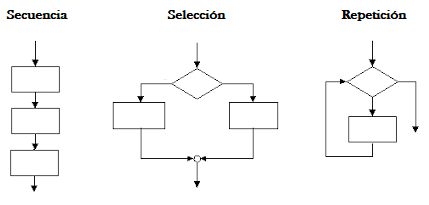
\includegraphics[scale=0.7]{images/pantalla3.png}
\end{center}
\end{frame}

\begin{frame}{Introducción}
\begin{center}
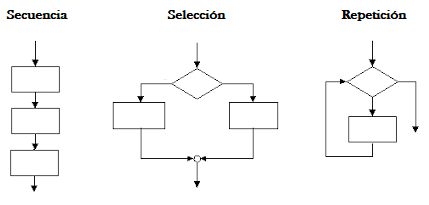
\includegraphics[scale=0.55]{images/pantalla3.png}
\end{center}
\begin{block}{Tener en cuenta}
Estructuras de selección y repetición dependen de operadores relacionales y lógico.
\end{block}
\end{frame}

\begin{frame}{Operadores relacionales}
\textbf{Operadores relacionales:}
\begin{table}[]
\centering
\begin{tabular}{|c|c|}
\hline
Operador relacional & Interpretación      \\ \hline
\textless{}         & Menor que           \\ \hline
\textless{}=        & Menor que o igual a \\ \hline
\textgreater{}      & Mayor que           \\ \hline
\textgreater{}=     & Mayor que o igual a \\ \hline
==                  & Igual a             \\ \hline
$\sim$=             & no igual a          \\ \hline
\end{tabular}
\end{table}
\end{frame}

\begin{frame}{Operadores relacionales}
Ej. Ejecutar las siguientes líneas. Obtener conclusiones.
 \lstinputlisting[xleftmargin=.5\textwidth]{scripts/ej1.m}
\end{frame}

\begin{frame}{Operadores relacionales}
Ej. Ejecutar las siguientes líneas. Obtener conclusiones.
 \lstinputlisting[xleftmargin=.5\textwidth]{scripts/ej1.m}
Las comparaciones pueden ser verdaderas ó falsas. 
\begin{itemize}
\item Valor positivo: Verdadero (true)
\item Valor cero: Falso (false)
\end{itemize}
\end{frame}

\begin{frame}{Operadores relacionales}
Ej. Ejecutar las siguientes líneas. Obtener conclusiones.
 \lstinputlisting[xleftmargin=.5\textwidth]{scripts/ej2.m}
\end{frame}

\begin{frame}{Operadores relacionales}
Ej. Ejecutar las siguientes líneas. Obtener conclusiones.
\lstinputlisting[xleftmargin=.5\textwidth]{scripts/ej2.m}
\begin{alertblock}{Tener en cuenta}
Para que una comparación sea verdadera, debe ser \textbf{verdadera} para cada elemento de la matriz.
\end{alertblock}
\end{frame}



\begin{frame}{Operadores lógicos}
\textbf{Operadores lógicos:}
\begin{table}[]
\centering
\begin{tabular}{|c|c|}
\hline
operador lógico & Interpretación \\ \hline
\&              & and            \\ \hline
$\sim$          & not            \\ \hline
|               & or             \\ \hline
\end{tabular}
\end{table}
\end{frame}

\begin{frame}{Operadores lógicos}
\textbf{Cómo leemos:}
\begin{columns}
\begin{column}{0.5\textwidth}
\begin{center}
\Huge (z>x)\&(z>y)
\end{center}
\end{column}
\begin{column}{0.5\textwidth}
\begin{center}

\includegraphics[scale=0.4]{images/img41.png}
\end{center}
\end{column}
\end{columns}
\end{frame}

\begin{frame}{Operadores lógicos}
Ej. Ejecutar las siguientes líneas. Obtener conclusiones.
\lstinputlisting[xleftmargin=.4\textwidth]{scripts/ej3.m}
\end{frame}

\begin{frame}{Estructura de selección - if}
\begin{columns}
\begin{column}{0.5\textwidth}
\begin{center}
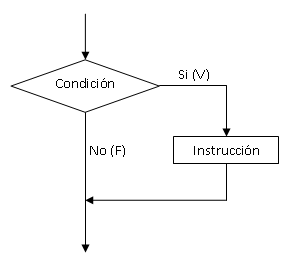
\includegraphics[scale=0.5]{images/pantalla5.png}
\end{center}
\end{column}
\begin{column}{0.5\textwidth}
\lstinputlisting[]{scripts/ej4.m}
\end{column}
\end{columns}
\begin{center}
Se ejecutan los comandos si y sólo si la condición es verdadera
\end{center}
\end{frame}

\begin{frame}{Estructura de selección - if/else}
\begin{columns}
\begin{column}{0.5\textwidth}
\begin{center}
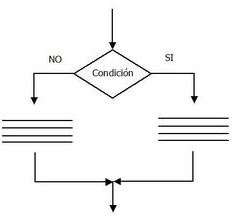
\includegraphics[scale=0.5]{images/pantalla4.png}
\end{center}
\end{column}
\begin{column}{0.5\textwidth}
\lstinputlisting[]{scripts/ej5.m}
\end{column}
\end{columns}
\begin{center}
Se ejecutan las instrucciones 1 si la condición es verdadera y las instrucciones 2 si la condición es falsa. 
\end{center}
\end{frame}

\begin{frame}{Estructura de selección - elseif}
\begin{columns}
\begin{column}{0.5\textwidth}
\begin{center}
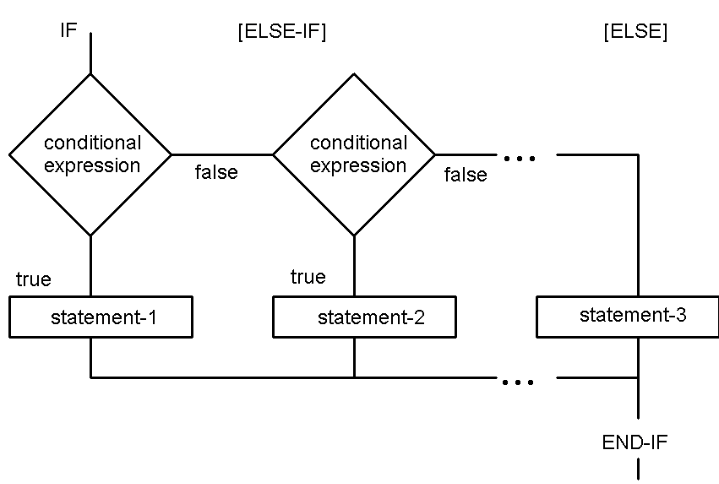
\includegraphics[scale=0.2]{images/pantalla6.png}
\end{center}
\end{column}
\begin{column}{0.5\textwidth}
\lstinputlisting[]{scripts/ej6.m}
\end{column}
\end{columns}
\end{frame}

\begin{frame}{Ejercicio práctico 11}
Escriba una función if para cada uno de los siguientes problemas si supone que la entrada a la función es un escalar.
\begin{enumerate}
\item Suponga que en un estado la edad legal para beber es 21. Escriba y pruebe una función para determinar si una persona es lo suficientemente madura para beber.
\item Cuando una parte se fabrica, las dimensiones usualmente se especifican con una tolerancia. Suponga que cierta parte necesita tener 5.4cm de largo, más o menos 0.1cm (5.4 +/- 0.1cm). Escriba una función para determinar si una parte está dentro de dichas especificaciones.
\end{enumerate}
\end{frame}

\begin{frame}{Estructura de selección - Switch/case}
Ejecuta ciertas sentencias basadas en el valor de una variable o expresión.
\begin{columns}
\begin{column}{0.5\textwidth}
\begin{center}
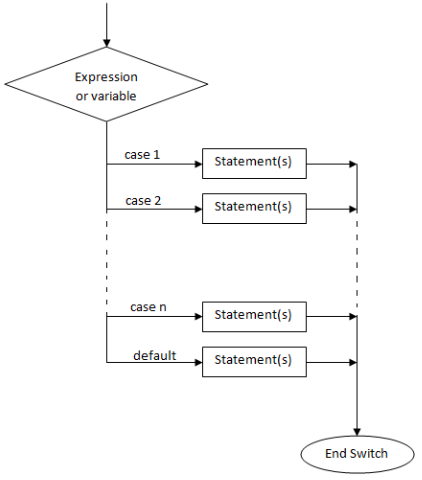
\includegraphics[scale=0.2]{images/pantalla7.png}
\end{center}
\end{column}
\begin{column}{0.5\textwidth}
\lstinputlisting[]{scripts/ej7.m}
\end{column}
\end{columns}

\begin{block}{Tener en cuenta}
\textbf{Otherwise} puede ser omitido.
\end{block}
\end{frame}

\begin{frame}{Menu}
\begin{exampleblock}{Comando}
Ver comando: \textbf{menu}
\end{exampleblock}

Ej. Ejecutar las siguientes líneas. Obtener conclusiones.
\lstinputlisting[xleftmargin=.1\textwidth]{scripts/menu.m}
\end{frame}

\begin{frame}{Ejercicio práctico 12}
\begin{enumerate}
\item Cree un programa que pida al usuario su año en la escuela: primero, segundo, tercero o cuarto. La entrada sera una cadena. Use la estructura switch/case para determinar qué día serán los finales para cada grupo: lunes para primero, martes para segundo, miércoles para tercero y jueves para cuarto.
\item Repita el problema 1 pero esta vez con un menú
\item Cree un programa que pida al usuario ingresar el número de dulces que le gustaría comprar. La entrada será un número. Use la estructura switch/case para determinar la cuenta, donde:
\begin{itemize}
\item 1 dulce = 0.75\$
\item 2 dulces = 1.25\$
\item 3 dulces = 1.65\$
\end{itemize}
más de 3 dulces = 1.65\$ + 0.3 * (número ordenado -3)
\end{enumerate}
\end{frame}

\begin{frame}{Estructura de repetición - for}
\begin{columns}
\begin{column}{0.5\textwidth}
\begin{center}
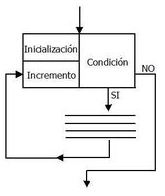
\includegraphics[scale=0.7]{images/pantalla8.png}
\end{center}
\end{column}
\begin{column}{0.5\textwidth}
\lstinputlisting[]{scripts/ej8.m}
\end{column}
\end{columns}
\begin{center}
Las instrucciones dentro del bucle for se repiten N veces.
\end{center}
\end{frame}

\begin{frame}{Ejercicio práctico 13}
Considere la siguiente matriz de valores: x = [45,23,17,34,85,33] determine cuántos elementos son mayores que 30 utilizando un contador. \textit{Ayuda: Utilice la función length().}
\end{frame}

\begin{frame}{Estructura de repetición - while}
Ejecutar un grupo de instrucciones mientras se cumpla una condición lógica
\begin{columns}
\begin{column}{0.5\textwidth}
\begin{center}
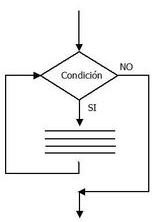
\includegraphics[scale=0.7]{images/pantalla9.png}
\end{center}
\end{column}
\begin{column}{0.5\textwidth}
\lstinputlisting[]{scripts/ej9.m}
\end{column}
\end{columns}
\end{frame}

\begin{frame}{Ejercicio práctico 14}
Considere la siguiente matriz de valores: x = [45,23,17,34,85,33] determine cuántos elementos son mayores que 30 utilizando un contador. \textit{Ayuda: Utilice la función length().}
\end{frame}

\begin{frame}{Instrucción break y continue}
\begin{columns}
\begin{column}{0.5\textwidth}
\begin{itemize}
\item La instrucción \textbf{break} finaliza la ejecución del bucle for o while. A continuación se ejecuta la siguiente instrucción fuera del bloque.
\item La instrucción \textbf{continue} pasa el control a la iteración siguiente en un bucle for o while.
\end{itemize}
\end{column}
\begin{column}{0.5\textwidth}
\begin{center}

\includegraphics[scale=0.3]{images/img40.png}
\end{center}
\end{column}
\end{columns}
\end{frame}

\end{document}
